\chapter{磁光阱装载实验}
本章将重点介绍磁光阱装载实验。激光冷却作为自20世纪80年代发展起来的一项核心冷原子实验技术，为冷原子物理研究提供了关键支撑。本实验采用二维磁光阱（2D MOT）对原子束流进行预冷却处理，随后通过差分管将预冷却后的原子束流送入三维磁光阱（3D MOT）中，最终形成稳定的冷原子团，为后续磁阱装载实验奠定基础。本章将首先系统阐述激光冷却与磁光阱的相关基本原理，随后呈现磁光阱装载的实验结果，并对实验现象及结果进行详细分析与讨论。
\section{激光冷却原理}
激光冷却主要利用光对原子的散射力效应。当静止原子吸收$N$个共振光子后，会通过自发辐射释放这些光子，由于自发辐射具有各向同性，其引起的动量变化相互抵消为零；根据动量守恒定律，原子在吸收光子时会获得相应的反冲动量。考虑到原子本身具有一定的运动速度，会产生多普勒效应，运动原子所观测到的激光频率相较于激光本征频率会发生偏移，当原子与激光相向运动时，需采用红失谐激光方可实现原子与光子的共振相互作用。在小速度近似范围内，原子将受到与运动方向相反、大小正比于速度的阻尼力，进而能够在对射激光场中实现冷却。
\begin{figure}[htbp]
	\centering
	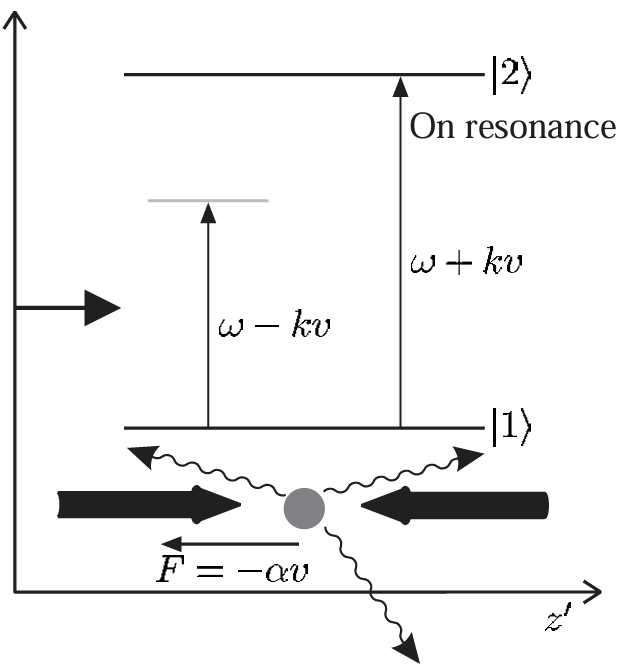
\includegraphics[width=0.4\linewidth]{figs/ch3-1.png}
	\caption{激光冷却原理图}
	\label{fig:ch3-1}
\end{figure}
随机行走计算
\begin{figure}[htbp]
	\centering
	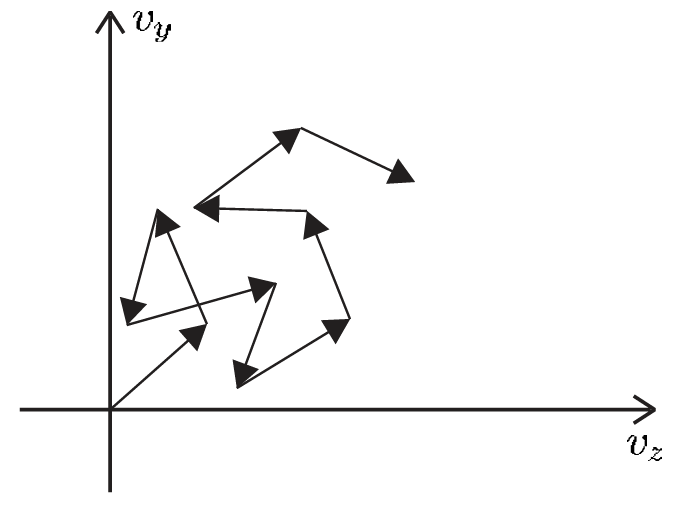
\includegraphics[width=0.4\linewidth]{figs/ch3-2.png}
	\caption{原子在光学黏团中的随机行走}
	\label{fig:ch3-2}
\end{figure}

\section{磁光阱原理}
\begin{figure}[htbp]
	\centering
	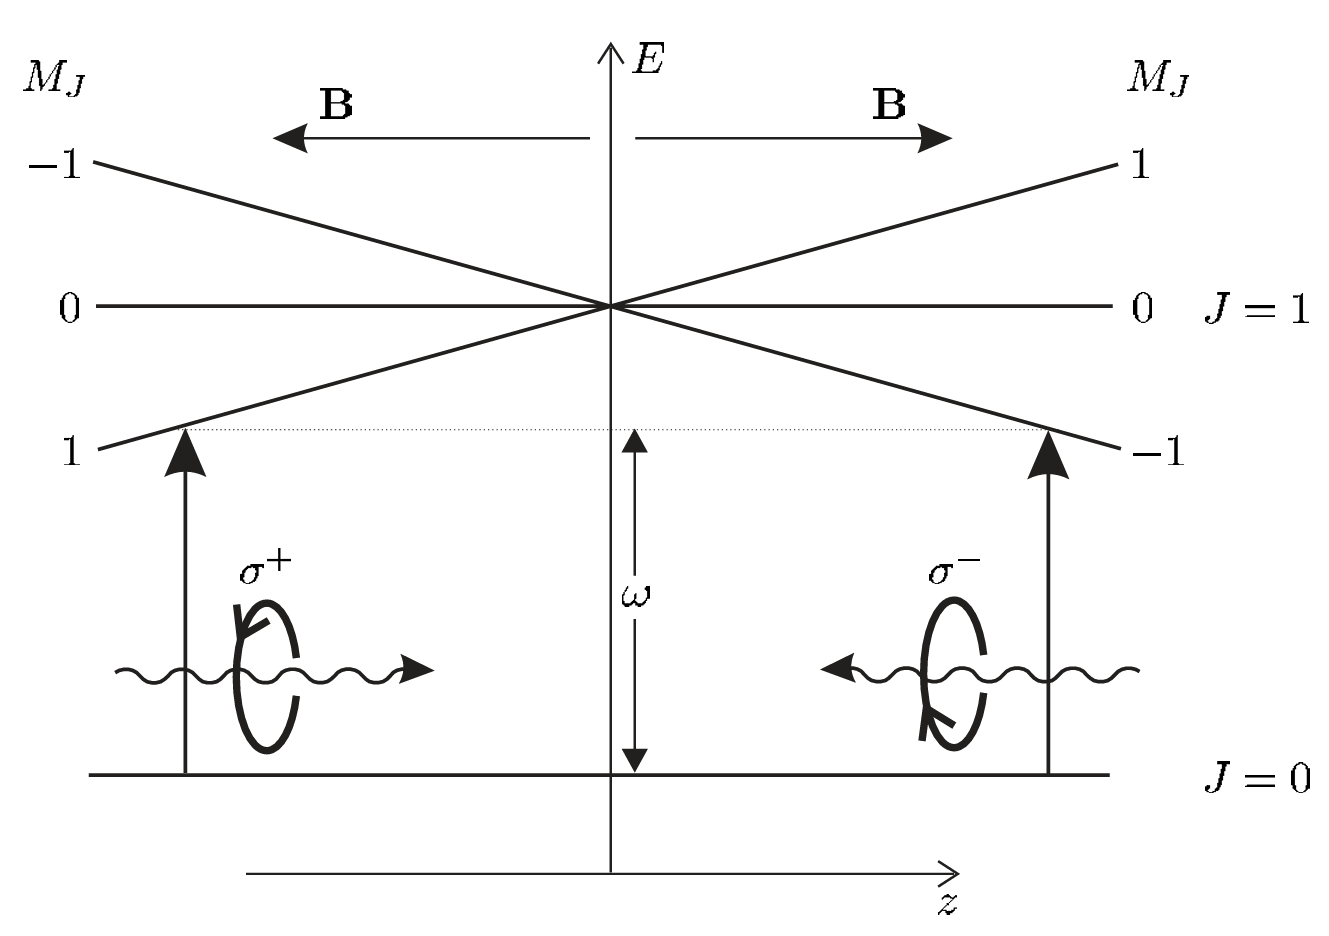
\includegraphics[width=0.4\linewidth]{figs/ch2-8.png}
	\caption{磁光阱原理图}
	\label{fig:ch2-8}
\end{figure}
\begin{figure}[htbp]
	\centering
	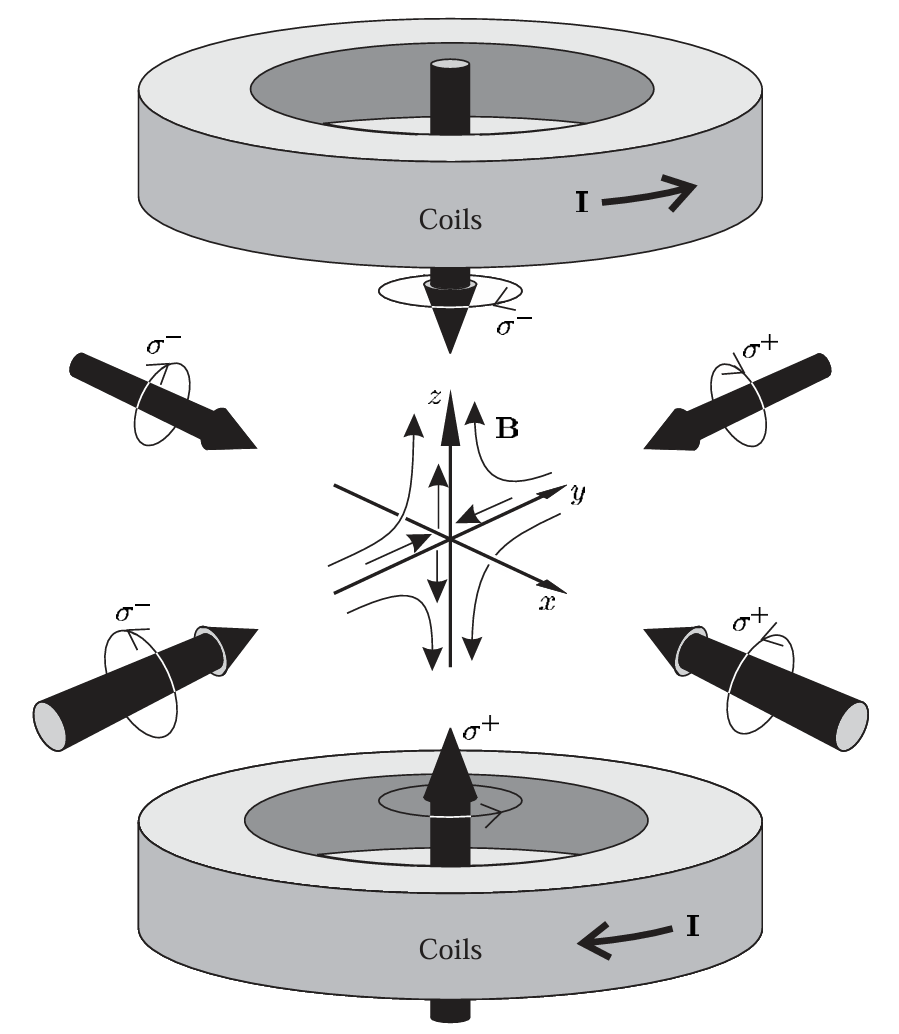
\includegraphics[width=0.4\linewidth]{figs/ch2-9.png}
	\caption{三维磁光阱立体图}
	\label{fig:ch2-9}
\end{figure}